Цель работы: Освоение возможностей программы Microsoft Project (MP) для планирования проекта по разработке программного обеспечения

\section{Задание 0}

Задание для тренировки. Номера вариант = номер в журнале Mod 4.
Номер варината: 1

Условие: Осуществить планирование проекта со следующими временными
характеристиками (таблица \ref{tab:var1})

\begin{table}[H]
	\caption{Вариант 1}
	\label{tab:var1}
	\begin{tabular}{|l|l|}
		\hline
		Название работы & Длительность (дни) \\
		\hline
		Работа А & 12 \\
		\hline
		Работа B & 6 \\
		\hline
		Работа C & 10 \\
		\hline
		Работа D & 7 \\
		\hline
		Работа E & 9 \\
		\hline
		Работа F & 8 \\
		\hline
		Работа G & 10 \\
		\hline
		Работа H & 10 \\
		\hline
		Работа I & 6 \\
		\hline
		Работа J & 5 \\
		\hline
	\end{tabular}
\end{table}

Дата начала проекта – 1-й рабочий день марта текущего года.
Провести планирование работ проекта, учитывая следующие связи между задачами:
\begin{enumerate}
	\item Предусмотреть, что D – исходная работа проекта;
	\item Работы С, E и F начинаются сразу по окончании работы D;
	\item Работы A и J следуют за C, а работа G – за F;
	\item Работа I следует за A, а работа B – за G
	\item Работа H начинается после завершения E, но не может начаться, пока не завершены I и B.
\end{enumerate}

\subsection{Результаты и настройки}

На рисунках \ref{fig:task01}, \ref{fig:task02}, \ref{fig:task03} отображены результаты работ и настройки среды.

\begin{figure}[H]
	\centering
	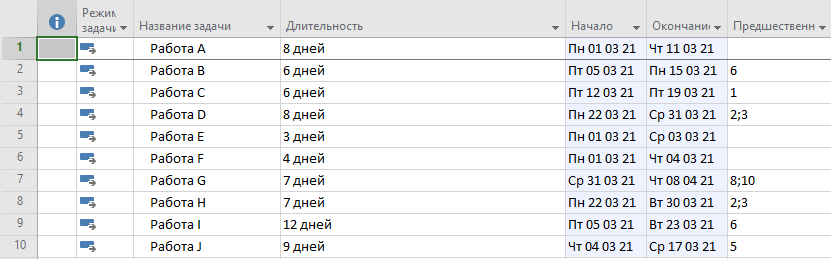
\includegraphics[width=0.7\linewidth]{src/task0_1}
	\caption{Даты начала и завершения работ}
	\label{fig:task01}
\end{figure}
\begin{figure}[H]
	\centering
	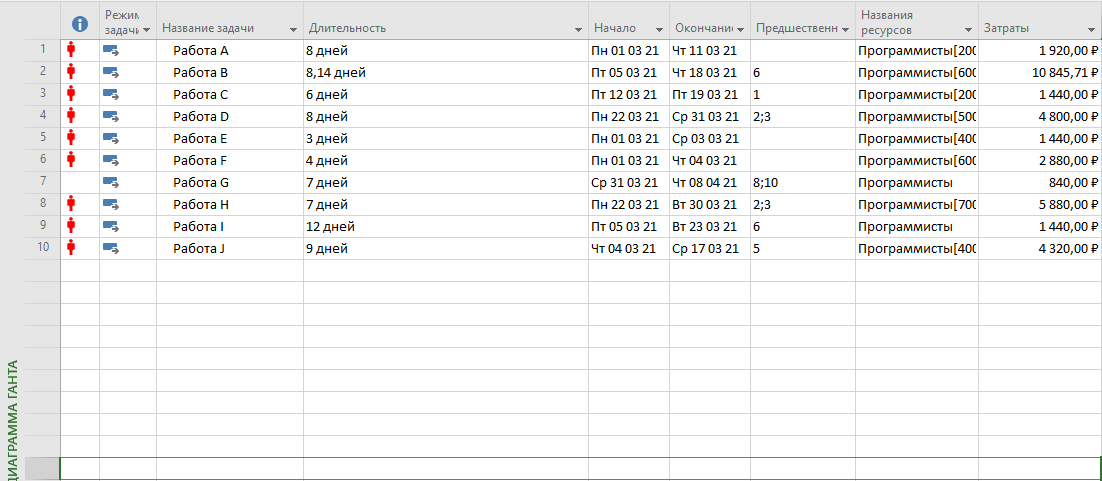
\includegraphics[width=0.7\linewidth]{src/task0_2}
	\caption{Диаграмма Ганта}
	\label{fig:task02}
\end{figure}
\begin{figure}[H]
	\centering
	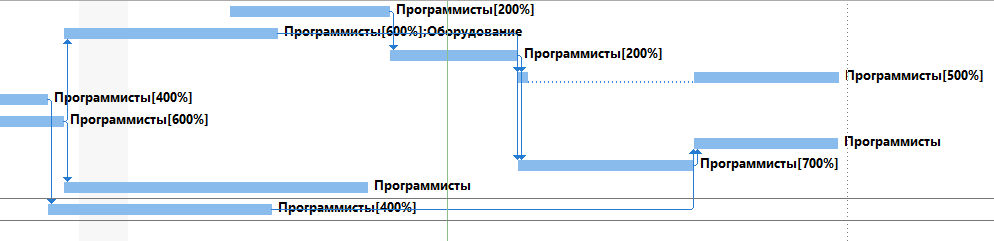
\includegraphics[width=0.7\linewidth]{src/task0_3}
	\caption{Настройки среды}
	\label{fig:task03}
\end{figure}

\section{Задание 1}
Настройка рабочей среды проекта

Подзадачи:
\begin{enumerate}
	\item Установите дату начала проекта - первый рабочий день марта текущего года \ref{fig:task11}.
	Для этого заходим в Проект -> Сведения о проекте и дату начала ставим на 01.03.21.
	\item Установите длительность работы в неделях, объем работ в часах, а тип работ по умолчанию- с фиксированными трудозатратами \ref{fig:task11}. Файл -> Параметры -> Расписание
	\item Установите количество рабочих часов в день равным 8, количество рабочих часов в неделю равным 40 \ref{fig:task12}. 
	Файл -> Параметры -> Расписание.
	\item Задайте начало рабочей недели в понедельник, а финансового года - в январе \ref{fig:task12}. 
	Файл -> Параметры -> Расписание. 
	\item Установите продолжительность рабочего дня с 9 до 18 часов \ref{fig:task12}.
	Файл -> Параметры -> Расписание.
	\item Установите стандартный календарь рабочего времени \ref{fig:task11}.
	Проект -> Сведения -> Календарь -> выбираем стандартный тип календаря
	\item Отметьте выходные и праздничные дни на ближайшие семь-восемь календарных месяцев от даты начала проекта.
	Проект -> Изменить рабочее время -> Выбираем необходимые даты в соглосовании с производственным календарем \ref{fig:task14} и ставим их как нерабочий день.
	Если день сокращенный, то ставим особые часы работы \ref{fig:task14}.
	\item Выведите на экран суммарную задачу проекта и заполните вкладку Заметки информацией об основных параметрах проекта (его длительности, бюджете и	количественном составе команды) \ref{fig:task15}.
\end{enumerate}
\begin{figure}[H]
	\centering
	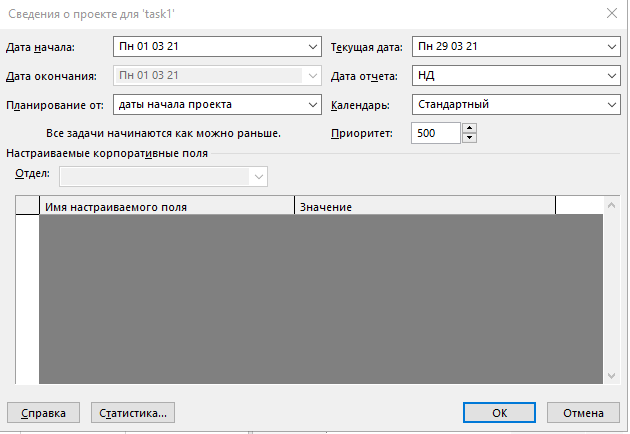
\includegraphics[width=0.7\linewidth]{src/task_1_1}
	\caption{Настройка проекта}
	\label{fig:task11}
\end{figure}
\begin{figure}[H]
	\centering
	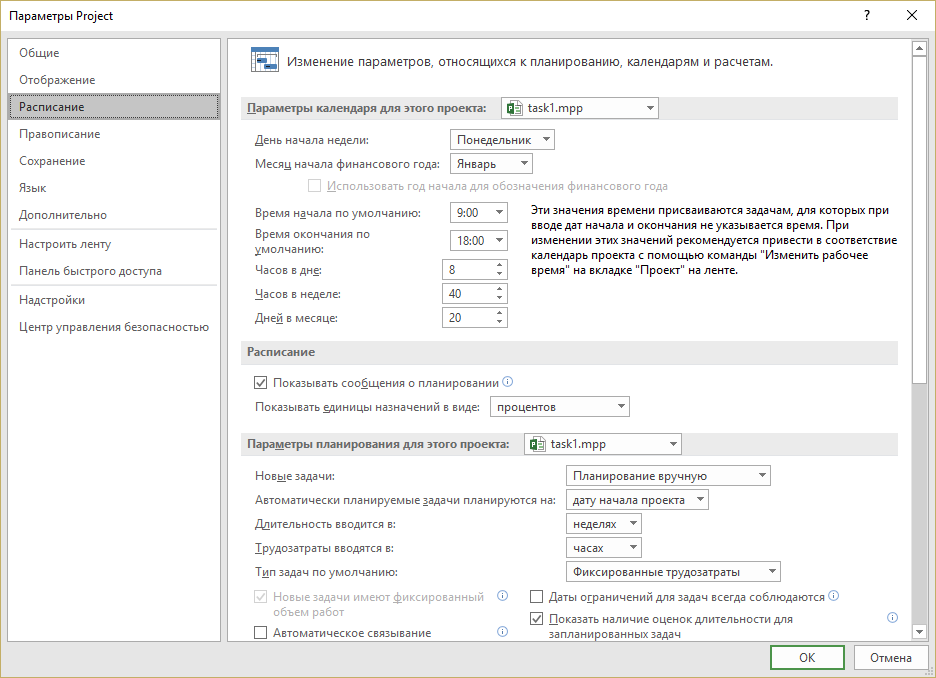
\includegraphics[width=0.7\linewidth]{src/task_1_2}
	\caption{Настройка среды проекта}
	\label{fig:task12}
\end{figure}
\begin{figure}[H]
	\centering
	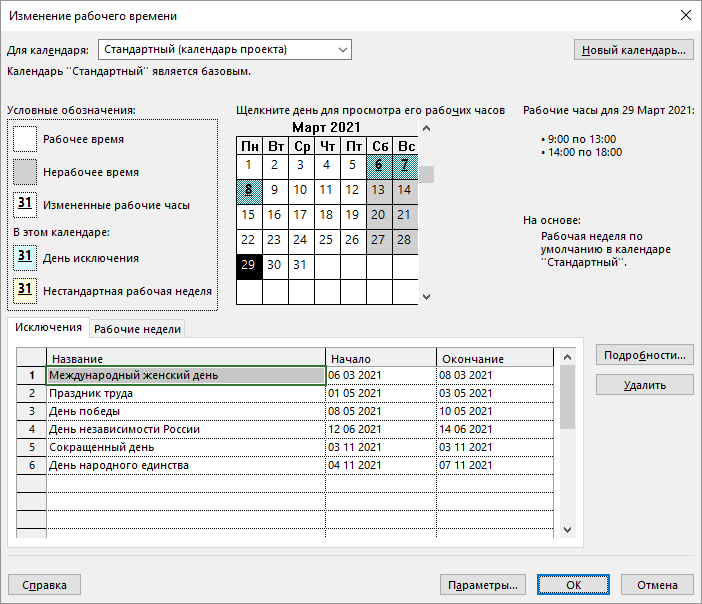
\includegraphics[width=0.7\linewidth]{src/task_1_3}
	\caption[Настройка праздников и выходных дней]{}
	\label{fig:task13}
\end{figure}
\begin{figure}[H]
	\centering
	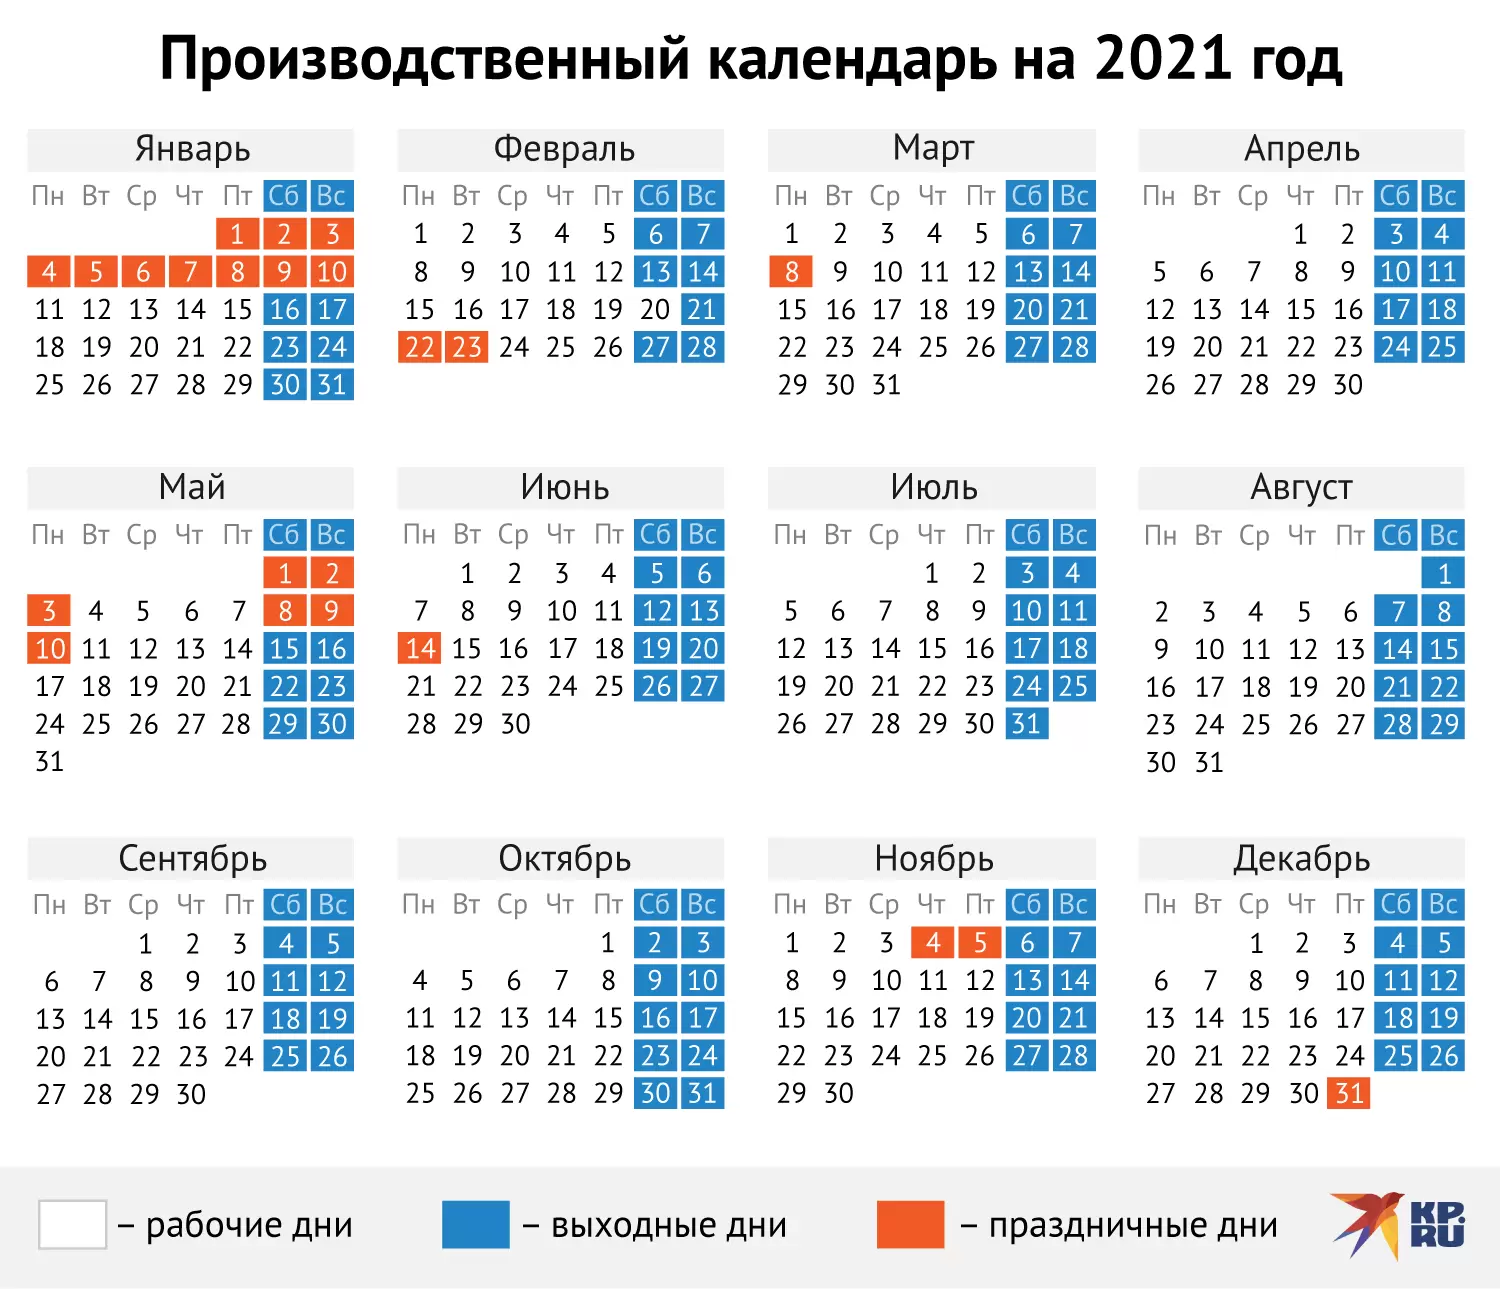
\includegraphics[width=0.7\linewidth]{src/task_1_4}
	\caption[Производственный календарь]{}
	\label{fig:task14}
\end{figure}
\begin{figure}[H]
	\centering
	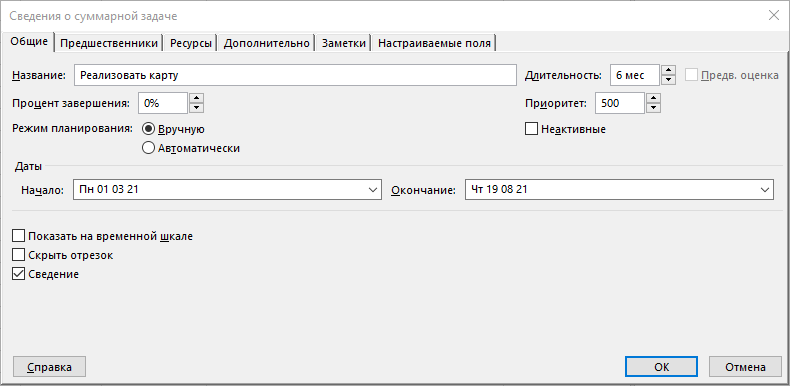
\includegraphics[width=0.7\linewidth]{src/task_1_5}
	\caption{Настройка ресурсов}
	\label{fig:task15}
\end{figure}

\section{Задание 2}

Ввести задачи в соответствии с таблицей \ref{fig:task16}
\begin{figure}[H]
	\centering
	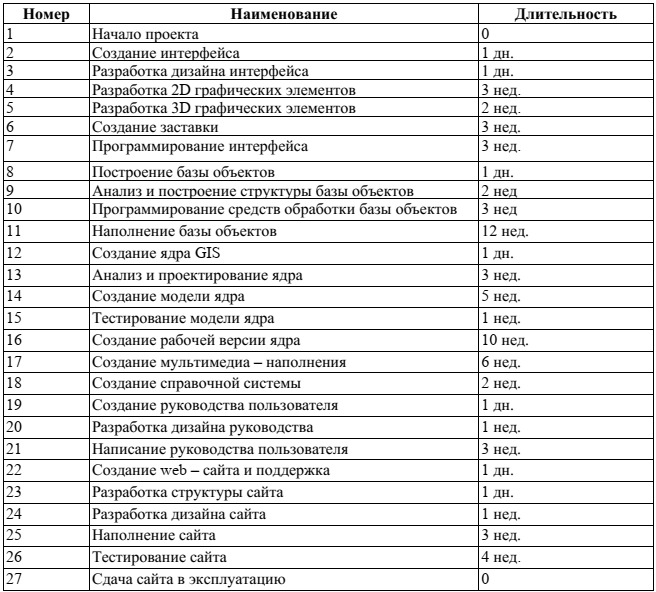
\includegraphics[width=0.7\linewidth]{src/task_1_6}
	\caption{Таблица задач}
	\label{fig:task16}
\end{figure}

\section{Задание 3}

Структурировать список задач. На изображении \ref{fig:task31} отображен результат.

\begin{figure}[H]
	\centering
	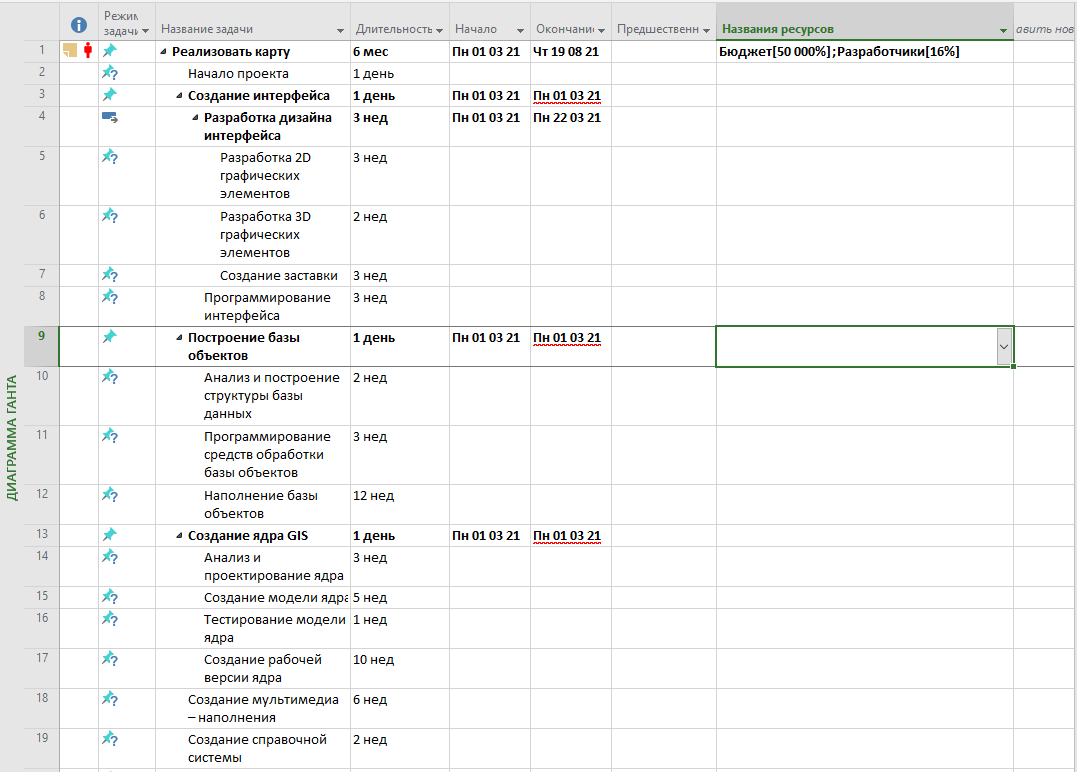
\includegraphics[width=0.7\linewidth]{src/task_3_1}
	\caption{Результат структуризации}
	\label{fig:task31}
\end{figure}

\section{Задание 4}

Установить связи между задачами.

\section{Вывод}
При выполнении лабораторной работы удалось познакомится с возможностями программы Microsoft Project. В рамках лабораторной работы был создан проект разработки ПО. Для него были введены задачи и подзадачи, для которых задана последовательность их выполнения с учётом типов связей.

По заданным условиям проект должен завершиться за 6 месяцев (24 недели) 19.08.21. В результате выполнения 4 задания было получено, что работы (в из зависимостях) завершатся 24.08.21. То есть с опозданием.






